\documentclass[10pt,a4paper,]{article}
\usepackage[]{mathpazo}
\usepackage{setspace}

\usepackage{amssymb,amsmath}
\usepackage{ifxetex,ifluatex}
\usepackage{fixltx2e} % provides \textsubscript
\ifnum 0\ifxetex 1\fi\ifluatex 1\fi=0 % if pdftex
  \usepackage[T1]{fontenc}
  \usepackage[utf8]{inputenc}
  \usepackage{csquotes}
\else % if luatex or xelatex
  \usepackage{unicode-math}
  \defaultfontfeatures{Ligatures=TeX,Scale=MatchLowercase}
\fi
% use upquote if available, for straight quotes in verbatim environments
\IfFileExists{upquote.sty}{\usepackage{upquote}}{}
% use microtype if available
\IfFileExists{microtype.sty}{%
\usepackage[]{microtype}
\UseMicrotypeSet[protrusion]{basicmath} % disable protrusion for tt fonts
}{}
\PassOptionsToPackage{hyphens}{url} % url is loaded by hyperref
\usepackage[unicode=true]{hyperref}
\hypersetup{
            pdftitle={Revisiting some definitions with common examples from Gregorian calendar},
            pdfauthor={Sayani Gupta},
            pdfborder={0 0 0},
            breaklinks=true}
\urlstyle{same}  % don't use monospace font for urls
\usepackage{geometry}
\geometry{left=2cm,right=2cm,top=2.5cm,bottom=2.5cm}
\usepackage[style=authoryear-comp,backend=biber, natbib=true,]{biblatex}
\usepackage{longtable,booktabs}
% Fix footnotes in tables (requires footnote package)
\IfFileExists{footnote.sty}{\usepackage{footnote}\makesavenoteenv{long table}}{}
\IfFileExists{parskip.sty}{%
\usepackage{parskip}
}{% else
\setlength{\parindent}{0pt}
\setlength{\parskip}{6pt plus 2pt minus 1pt}
}
\setlength{\emergencystretch}{3em}  % prevent overfull lines
\providecommand{\tightlist}{%
  \setlength{\itemsep}{0pt}\setlength{\parskip}{0pt}}
\setcounter{secnumdepth}{5}

% set default figure placement to htbp
\makeatletter
\def\fps@figure{htbp}
\makeatother

\title{Revisiting some definitions with common examples from Gregorian calendar}

\author{Sayani Gupta}

%% MONASH STUFF

%% CAPTIONS
\RequirePackage{caption}
\DeclareCaptionStyle{italic}[justification=centering]
 {labelfont={bf},textfont={it},labelsep=colon}
\captionsetup[figure]{style=italic,format=hang,singlelinecheck=true}
\captionsetup[table]{style=italic,format=hang,singlelinecheck=true}

%% FONT
\usepackage{bm,url}

%% HEADERS AND FOOTERS
\RequirePackage{fancyhdr}
\pagestyle{fancy}
\lfoot{}\cfoot{}\rfoot{}
\lhead{\textsf{Revisiting some definitions with common examples from Gregorian calendar}}
\rhead{\textsf{\thepage}}
\setlength{\headheight}{15pt}
\renewcommand{\headrulewidth}{0.4pt}
\fancypagestyle{plain}{%
\fancyhf{} % clear all header and footer fields
\fancyfoot[C]{\sffamily\thepage} % except the center
\renewcommand{\headrulewidth}{0pt}
\renewcommand{\footrulewidth}{0pt}}

%% MATHS
\RequirePackage{bm,amsmath}
\allowdisplaybreaks

%% GRAPHICS
\RequirePackage{graphicx}
\RequirePackage{float}
\setcounter{topnumber}{2}
\setcounter{bottomnumber}{2}
\setcounter{totalnumber}{4}
\renewcommand{\topfraction}{0.85}
\renewcommand{\bottomfraction}{0.85}
\renewcommand{\textfraction}{0.15}
\renewcommand{\floatpagefraction}{0.8}

%\RequirePackage[section]{placeins}

%% SECTION TITLES
\RequirePackage[compact,sf,bf]{titlesec}
\titleformat{\section}[block]
  {\fontsize{15}{17}\bfseries\sffamily}
  {\thesection}
  {0.4em}{}
\titleformat{\subsection}[block]
  {\fontsize{12}{14}\bfseries\sffamily}
  {\thesubsection}
  {0.4em}{}
\titlespacing{\section}{0pt}{*3}{*1}
\titlespacing{\subsection}{0pt}{*1}{*0.5}

%% LINE AND PAGE BREAKING
\sloppy
\raggedbottom
\usepackage[bottom]{footmisc}
\clubpenalty = 10000
\widowpenalty = 10000
\brokenpenalty = 10000
\RequirePackage{microtype}

%% HYPERLINKS
\RequirePackage{xcolor} % Needed for links
\definecolor{darkblue}{rgb}{0,0,.6}
\RequirePackage{url}

\makeatletter
\@ifpackageloaded{hyperref}{}{\RequirePackage{hyperref}}
\makeatother
\hypersetup{
     citecolor=0 0 0,
     breaklinks=true,
     bookmarksopen=true,
     bookmarksnumbered=true,
     linkcolor=darkblue,
     urlcolor=blue,
     citecolor=darkblue,
     colorlinks=true}

\usepackage[showonlyrefs]{mathtools}

%% BIBLIOGRAPHY

\makeatletter
\@ifpackageloaded{biblatex}{}{\usepackage[style=authoryear-comp, backend=biber, natbib=true]{biblatex}}
\makeatother
\ExecuteBibliographyOptions{bibencoding=utf8,minnames=1,maxnames=3, maxbibnames=99,dashed=false,terseinits=true,giveninits=true,uniquename=false,uniquelist=false,doi=false, isbn=false,url=true,sortcites=false}
\DeclareFieldFormat{url}{\texttt{\url{#1}}}
\DeclareFieldFormat[article]{pages}{#1}
\DeclareFieldFormat[inproceedings]{pages}{\lowercase{pp.}#1}
\DeclareFieldFormat[incollection]{pages}{\lowercase{pp.}#1}
\DeclareFieldFormat[article]{volume}{\mkbibbold{#1}}
\DeclareFieldFormat[article]{number}{\mkbibparens{#1}}
\DeclareFieldFormat[article]{title}{\MakeCapital{#1}}
\DeclareFieldFormat[article]{url}{}
%\DeclareFieldFormat[book]{url}{}
%\DeclareFieldFormat[inbook]{url}{}
%\DeclareFieldFormat[incollection]{url}{}
%\DeclareFieldFormat[inproceedings]{url}{}
\DeclareFieldFormat[inproceedings]{title}{#1}
\DeclareFieldFormat{shorthandwidth}{#1}
%\DeclareFieldFormat{extrayear}{}
% No dot before number of articles
\usepackage{xpatch}
\xpatchbibmacro{volume+number+eid}{\setunit*{\adddot}}{}{}{}
% Remove In: for an article.
\renewbibmacro{in:}{%
  \ifentrytype{article}{}{%
  \printtext{\bibstring{in}\intitlepunct}}}
\AtEveryBibitem{\clearfield{month}}
\AtEveryCitekey{\clearfield{month}}
\makeatletter
\DeclareDelimFormat[cbx@textcite]{nameyeardelim}{\addspace}
\makeatother
\renewcommand*{\finalnamedelim}{%
  %\ifnumgreater{\value{liststop}}{2}{\finalandcomma}{}% there really should be no funny Oxford comma business here
  \addspace\&\space}

%%% Change title format
\usepackage{fancybox,color}
\usepackage[absolute,overlay]{textpos}
\setlength{\TPHorizModule}{1cm}
\setlength{\TPVertModule}{1cm}
\usepackage{titling}

\pretitle{%

\vspace*{-1cm}

\LARGE\bfseries}
\posttitle{\vspace*{0.3cm}\par}
\preauthor{\large}
\postauthor{\hfill}
\predate{\small}
\postdate{\vspace*{0.1cm}}

\newenvironment{fminipage}%
{\begin{Sbox}\begin{minipage}{\textwidth}}%
{\end{minipage}\end{Sbox}\colorbox[gray]{0.8}{\TheSbox}}
\raggedbottom

\usepackage[australian]{babel}
\date{\today}

\usepackage[lf,t]{carlito}
\titleformat{\section}[block]{\fontsize{12}{14}\bfseries\sffamily}{\thesection}{0.4em}{}
\def\mod{\text{~mod~}}


\begin{document}
\vspace*{-2cm}
\begin{fminipage}\sffamily
\maketitle
\end{fminipage}\vspace*{0.5cm}
\setstretch{1.2}


\hypertarget{groups-periodically}{%
\section{Groups-periodically}\label{groups-periodically}}

The concept already existed in the literature. This is an attempt to demystify the notations using the linear granularities day and month.

The grouping (day, month) has a period of 1 year. Ignoring leap years, this would mean that the behavior of days within months repeat every 365 days. That is, each month would consist of the same number of days in every year. We assume there are D linear granularity \enquote{day} and M linear granularity \enquote{month} in total.

\begin{equation}\label{eq:eq1}
\begin{split}
month(0) & = day(0)\bigcup day(1)\dots\bigcup day(30)\\
month(1) & = day(31)\bigcup day(32)\dots\bigcup day(58)\\
month(2) & = day(59)\bigcup day(60)\dots\bigcup day(89)\\
\dots\\
month(11) & = day(334)\dots day(363)\bigcup day(364)\\
\end{split}
\end{equation}

If we know the composition of each of the months in terms of days for one year, we can find the composition of any month beyond 1 year since the \enquote{pattern} repeats itself along the time domain due to the periodic property.

In other words, if
\begin{equation}\label{eq:eq2}
month(j) = day(a_1)\bigcup day(a_2)\dots\bigcup day(a_k) \quad for \quad j \in {0,1, 2, \dots, 11}
\end{equation}
then,\\
\begin{equation}
month(j + R) = day(a_1 + P)\bigcup day(a_2 + P)\dots\bigcup day(a_k + P) \quad for \quad j + R \leq M
\end{equation}

Here, P = 365 and R = 12 will have the meaning of the period of the grouping (day, month) and the number of months in each of these periods.

Generalizing it to any two linear granularities \(G\) and \(H\) , the formal way of defining the property \enquote{groups periodically into} would like the following:

\newtheorem{definition}{Definition}
\begin{definition}\label{def:periodical}
A granularity H is periodical with respect to a granularity $G$ if
(1) $G \trianglelefteq H$, and \\
(2) there exist $R,P \epsilon Z+$, where R is less than the number of granules of H, such
that for all $j \epsilon Z$, if $H(j) = \bigcup_{i \in S}G(i)$ and $H (j + R) \neq \phi$ then
$H (j + R) = \bigcup_{i \in S} G(i + P)$.
\end{definition}

Another way to represent \autoref{eq:eq1}

\begin{equation}\label{eq:eq3}
\begin{split}
month(0) & = \bigcup_{i \in S_0}day(i), \quad S_0 = {0, 1, 2, \dots, 30}\\
month(1) & = \bigcup_{i \in S_1}day(i), \quad S_1 = {31, 32, \dots, 58}\\
month(2) & = \bigcup_{i \in S_2}day(i), \quad S_2 = {59, 60, \dots, 89}\\
\vdots\\
month(11) &  = \bigcup_{i \in S_{11}}day(i), \quad S_{11} = {334, 335, \dots, 364}\\
\end{split}
\end{equation}

Here, \({S_0,...,S_{11}}\) are the sets of indexes of \(G\) describing \(month(0), . . . , month(11)\). Then from Definition \autoref{def:periodical}, it also follows that if \(H\) is periodical with respect to \(G\), then

\begin{equation}\label{eq:eq4}
H(j) = \bigcup_{i \in S_{j \text{~mod~}R}}G(P*\lfloor j/R \rfloor + i), 
\end{equation},

where \({S_0,...,S_{R-1}}\) are the sets of indexes of \(G\) describing \(H (0), . . . , H (R - 1)\) respectively. Here \((j \text{~mod~}R)\) represents the index among those in \({0, 1, \dots, R-1}\) that must be shifted to obtain \(H(j)\). The number of periods each granule of \(G\) composing \(H(j \text{~mod~}R)\) should be shifted is given by \(\lfloor j/R\rfloor\).

Thus, to obtain \(month(13)\) in terms of days we can either use Definition \autoref{def:periodical} or \autoref{eq:eq4}

\begin{equation}
\begin{split}
month(13) & =  month (1 + 12)\\
 & = \bigcup_{i \in S_1} day(i + 365) \quad since \quad month(1) =  \bigcup_{i \in S_1}day(i), \quad S_1 = {31, 32, \dots, 58}\\
 & = day(31 + 365)\bigcup day(32 + 365)\bigcup day(58 + 365)\\
\end{split}
\end{equation}

\begin{equation}
\begin{split}
month(13) & = \bigcup_{i \in S_{13 \text{~mod~}12}}day(365*\lfloor 13/12 \rfloor + i)\\
 & = \bigcup_{i \in S_1}day(365*1 + i)\\
 & = day(31 + 365)\bigcup day(32 + 365)\bigcup day(58 + 365)\\
\end{split}
\end{equation}

\hypertarget{circular-periodic-linear-granularities-regular-mapping}{%
\section{Circular (Periodic linear granularities + regular mapping)}\label{circular-periodic-linear-granularities-regular-mapping}}

A \textbf{circular} granularity can be defined using modular arithmetic due to its regular mapping with the bottom granularity. They are formed with linear granularities, one of which \enquote{groups periodically into} the other. In the following definition, we would assume that bottom granularity \(B\) groups periodically into \(G\) and number of granules of \(B\) in each granule of \(G\) is constant. Thus, if \(P\) and \(R\) have the meaning of the period of the grouping \((B, G)\) and the number of granules of \(G\) in each of these periods, then for circular granularity, \(P/R \in \mathbb{Z}^+\). Also, since each granule of \(G\) has same number of granules of \(B\), \(R\) can be taken to be \(1\) and \(P\) can be interpreted as the number of granules of B in any granule of G.

\begin{definition}\label{def:circular}
A circular granularity C(B, G) relates a linear granularity $G$ to the bottom granularity B, if

\begin{equation} \label{eq:eq5}
\begin{split}
C_{B, G}(z) & = {L}(z\text{~mod~}P) \quad \forall z \in \mathbb{Z}^+ \\
\end{split}
\end{equation}
where
z denotes the index set,
B denotes a full-integer labelled bottom granularity which groups periodically into linear granularity $G$ with regular mapping, 
{L} is a label mapping that defines an unique label for each index $l \in {0,1,\dots, (P-1)}$,
and P is the number of granules of B in each granule of G.
\end{definition}

In general, the set of labels will be a set of strings that is more descriptive than the index and used to identify a categorization of the circular granularity. However, the labels can coincide with indexes in which case integers are directly used to refer to categorizations of the circular granularity. Note that each
circular granularity can use different label mappings. In \autoref{fig:day-of-week}, the label mapping L can be defined as \(L: ({0,1,2, \dots, 6}) \longmapsto\ ({Sun, Mon, \dots, Sat)}\) or \(L: ({0,1,2, \dots, 6}) \longmapsto\ ({Sunday, Monday, \dots, Saturday)}\) or \(L: ({0,1,2, \dots, 6}) \longmapsto\ ({0, 1, \dots, 6)}\)
depending on the context.

\begin{figure}
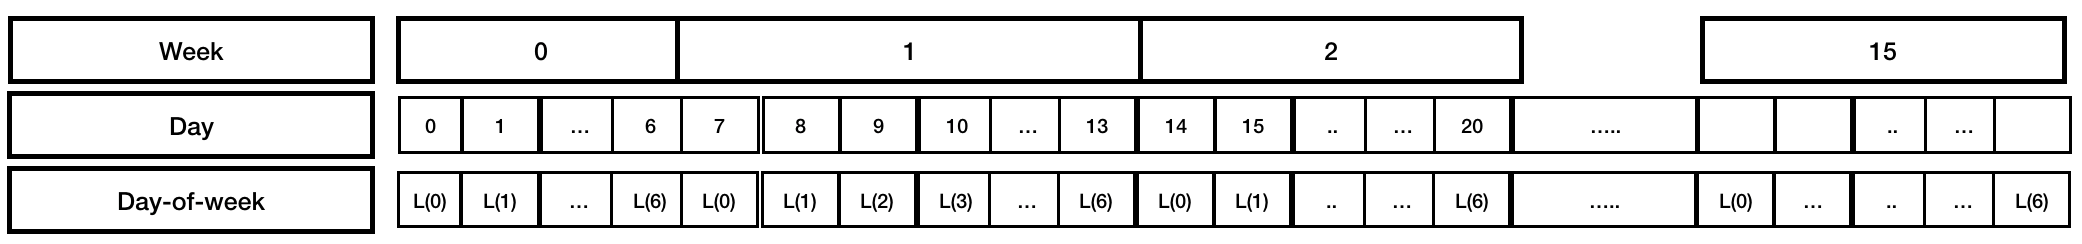
\includegraphics[width=1\linewidth]{Figs/day-of-week} \caption{Circular granularity day-of-week}\label{fig:day-of-week}
\end{figure}

\hypertarget{quasi-circular-periodic-linear-granularities-irregular-mapping}{%
\section{Quasi-circular (Periodic linear granularities + irregular mapping)}\label{quasi-circular-periodic-linear-granularities-irregular-mapping}}

A \textbf{quasi-circular} granularity can not be defined using modular arithmetic due to its irregular mapping with the bottom granularity. However, they are still formed with linear granularities, one of which \enquote{groups periodically into} the other. We shall discuss an example of quasi-circular granularity day-of-month in \autoref{fig:quasi-circular-explain}. The index 34 should correspond to L(3) which is \enquote{4th-day-of-month}, that of 60 should correspond to L(1), which is \enquote{2nd-day-of-month} and 334 should correspond to L(0), which is \enquote{1st-day-of-month}. Now, quasi-circular granularities can be defined as follows to manipulate the indices to our need:

\begin{figure}
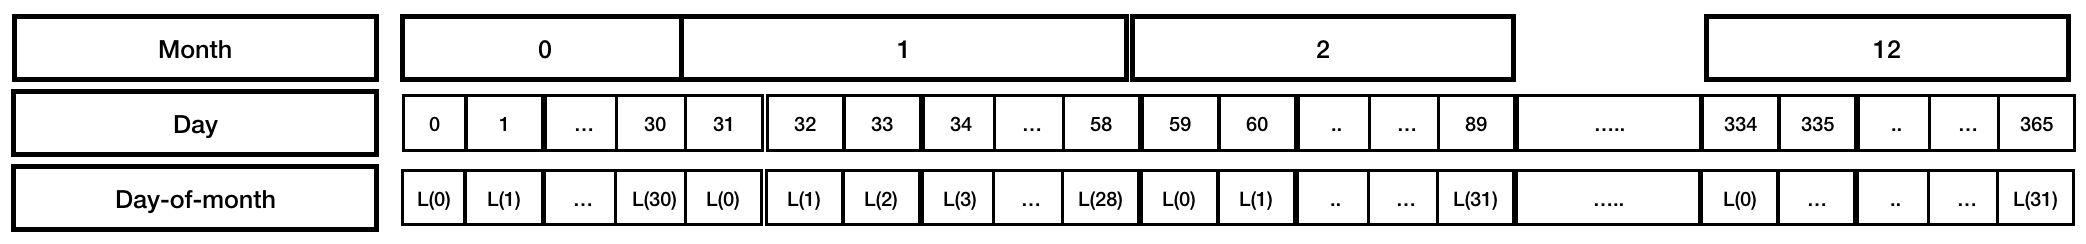
\includegraphics[width=1\linewidth]{Figs/quasi-circular-explain} \caption{Quasi-circular granularity day-of-month}\label{fig:quasi-circular-explain}
\end{figure}

\begin{definition}\label{quasicircular}
A quasi-circular granularity $Q_{B, G'}$ that relates linear granularities $G'$ and bottom granularity $B$, if

\begin{equation}\label{eq:eq6}
Q_{B, G'}(z) = L(z - \sum_{w=0}^{k-1}\vert T_{w \text{~mod~}R'} \vert), \quad z \in T_k
\end{equation}

where
$z$ denotes the index set,
$B$ denotes a full-integer labelled bottom granularity which groups periodically into linear granularity $G'$ with irregular mapping, {L} is a label mapping that defines an unique label for each index $l \in {0,1,\dots, (k-1)}$, $T_w$ are the sets of indices of B describing $G'(w)$ such that 
\begin{equation}
G'(w) = \bigcup_{z \in T_w}B(z),\\
\end{equation}
$T_w = 0 \quad for \quad w\epsilon Z_{<0}$ and $\vert T_w \vert$ is the cardinality of set $T_w$.
\end{definition}

Here, \(\vert T_w \vert\) = \(\vert T_{w\text{~mod~}R'} \vert\) since every \(w^{th}\) and \((w+R)^{th}\) granule will have the same number of granules of B. \(T_w\) are the sets of indexes of \(B\) describing \(G'(0), . . . , G'(R'- 1)\). The term \(\sum_{w=0}^{k-1}\vert T_{w \text{~mod~}R'}\vert\) denotes the number of granules of \(B\) till the \((k-1)^{th}\) granule of \(G'\).

In \autoref{fig:quasi-circular-explain}, the label mapping L can be defined as \(L: ({0,1,2, \dots, 31}) \longmapsto\ ({DOM_1, DOM_2, \dots, DOM_{31})}\) or \(L: ({0,1,2, \dots, 31}) \longmapsto\ ({1, 2, \dots, 31)}\)
depending on the context.

\begin{equation}
\begin{split}
Q_{day, month}(34) & = L(34 - 31)       = L(3) \quad since \quad 35 \in \quad month(1)\\
Q_{day, month}(60) & = L(60 - 31 - 28)  = L(2) , \quad since\quad 60 \in \quad month(2)\\
Q_{day, month}(334) & = L(334 - 334)    = L(0) \quad since \quad 334 \in \quad month(11)\\
Q_{day, month}(439) & = L(439 - \sum_{w=0}^{14-1}\vert T_{w \text{~mod~}12} \vert)\quad since \quad 439 \in \quad month(14)\\
& = L(439 - \sum_{w=0}^{13}\vert T_{w \text{~mod~}R'} \vert)\\
&  = L(439 - (2\vert T_{0} \vert + 2\vert T_{1}\vert + \vert T_{3}\vert + \vert T_{4}\vert + \dots + \vert T_{11}\vert))\\
&  = L(439 - 2\times 31 - 2\times 28 - 31 - 30 - \dots - 30)\\
&  = L(439 - 423)\\
&  = L(6)
\end{split}
\end{equation}.

The idea is we can find any day of the month beyond 1 year provided we have the composition of days across months in one year due to the periodic property.

\hypertarget{aperiodic-aperiodic-linear-granularities}{%
\section{Aperiodic (Aperiodic linear granularities)}\label{aperiodic-aperiodic-linear-granularities}}

\begin{definition}\label{aperiodic}
An aperiodic granularity $A_{B, G''}$ that relates linear granularities $G''$ and bottom granularity $B$, with $G''$ being aperiodical with respect to $B$, is given by

\begin{equation}\label{eq:eq7}
\begin{split}
A_{B, G''}(z) & = L(1), \quad z \in T_q\\
     & = L(0), \quad z \not\in T_q\\
\end{split}
\end{equation}
where  
$z$ denotes the index set,
$T_q$ are the sets of indices of $B$ describing $G''(q)$ such that $$G''(q) = \bigcup_{z \in T_q}B(z)$$
\end{definition}

Aperiodic time granularities map a time index to binary categories. It takes a value (eg. 1) whenever the time index coincides with the events in context (e.g.~public or school holiday) and another value 0 (e.g.~0) when it does not. \autoref{fig:aperiodic} shows the linear granularity academic semester and days. Academic semesters are not periodic with respect to days. The label mapping L can be defined as \(L: ({0,1}) \longmapsto\ ({On, Off)}\) or can be customized based on context.

\begin{figure}
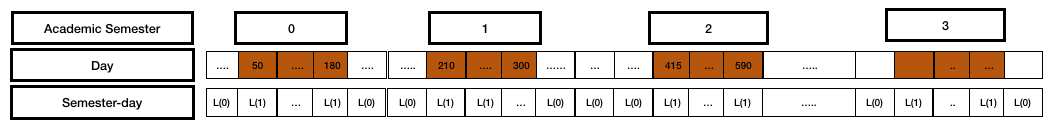
\includegraphics[width=1\linewidth]{Figs/academ-semester} \caption{ Aperiodic granularity day-semester}\label{fig:aperiodic}
\end{figure}

\printbibliography

\end{document}
